\setcounter{section}{0}
\section{BẤT ĐẲNG THỨC}
\subsection{Trọng tâm kiến thức}
\begin{tomtat}
\subsubsection{Bất đẳng thức}
Khi biểu diễn số thực trên trục số, điểm biểu đến số bé hơn nằm trước điểm biểu diễn số lớn hơn. Chẳng hạn, $-2{,}5<-1<1{,}5$.
\begin{center}
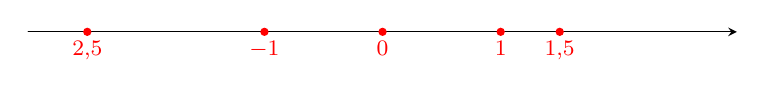
\begin{tikzpicture}[>=stealth,line join=round,line cap=round,font=\footnotesize,x=1.5cm]
\draw[->] (-3,0)--(3,0);
\foreach \x/\so in{-2.5/2{,}5,-1/-1,0/0,1/1,1.5/1{,}5}{
	\fill[red] (\x,0) circle (1.5pt) node[below]{$\so$};
}	
\end{tikzpicture}
\end{center}
\begin{itemize}
	\item Số $a$ lớn hơn hoặc bằng số $b$, tức là $a>b$ hoặc $a=b$, kí hiệu là $a\geq b$.
	\item Số $a$ nhỏ hơn hoặc bằng số $b$, tức là $a<b$ hoặc $a=b$, kí hiệu là $a\leq b$.
\end{itemize}
\begin{boxdn}
	Ta gọi hệ thức dạng $a>b$ (hay $a<b$, $a\geq b$, $a<\leq b$) là bất đẳng thức và gọi $a$ là vế trái, $b$ là vế phải của bất đẳng thức.
\end{boxdn}
\subsubsection{Tính chất bất đẳng thức}
\paragraph{Tính chất bắc cầu}
\begin{boxdn}
	\begin{tc}
	Cho ba số $a$, $b$, $c$. Nếu $a>b$ và $b>c$ thì $a>c$ (tính chất bắc cầu).
	\end{tc}
\end{boxdn}
\begin{note}
	Tính chất này vẫn đúng với các bất đẳng thức có dấu $<$, $\geq$, $\leq$.
\end{note}
\paragraph{Tính chất liên hệ thứ tự và phép cộng}
\begin{boxdn}
	\begin{itemize}
	\item Hai bất đẳng thức $a>b$ và $m>n$ được gọi là hai bất đẳng thức \textit{cùng chiều}.
	\item Hai bất đẳng thức $a>b$ và $m<n$ được gọi là hai bất đẳng thức \textit{ngược chiều}.
	\end{itemize}
	\textbf{Ta thấy:} Khi cộng cùng một số vào cả hai vế của một bất đẳng thức thì được một bất đẳng thức mới \textit{cùng chiều} với bất đẳng thức đã cho.\\
	Một cách tổng quát, ta có:
	\begin{tc}
	Cho ba số $a$, $b$, $c$. Nếu $a>b$ thì $a+c>b+c$.
	\end{tc}
\end{boxdn}
\begin{note}
	Tính chất này vẫn đúng với các bất đẳng thức có dấu $<$, $\geq$, $\leq$.
\end{note}
\paragraph{Tính chất liên hệ thứ tự và phép nhân}
\begin{boxdn}
	Khi nhân hai vế của một bất đẳng thức với cùng một \textbf{\textit{số dương}} thì được một bất đẳng thức mới \textbf{\textit{cùng chiều}} với bất đẳng thức đã cho.\\	
	Khi nhân hai vế của một bất đẳng thức với cùng một \textbf{\textit{số âm}} thì được một bất đẳng thức mới \textbf{\textit{ngược chiều}} với bất đẳng thức đã cho.\\
	Một cách tổng quát, ta có:
	\begin{tc}
	Cho ba số $a$, $b$, $c$ và $a>b$.
	\begin{itemize}
	\item Nếu $c>0$ thì $a\cdot c > b\cdot c$;
	\item Nếu $c<0$ thì $a\cdot c < b\cdot c$.
	\end{itemize}
	\end{tc}
\end{boxdn}
\begin{note}
	Tính chất này vẫn đúng với các bất đẳng thức có dấu $<$, $\geq$, $\leq$.
\end{note}	
\end{tomtat}
%%%%%%%%%%%%%%%%%%%%
\subsection{Các dạng bài tập}
\begin{dang}{Viết bất đẳng thức và một số yếu tố liên quan}
\end{dang}
%%==========Ví dụ 1
\begin{vd}
	Hãy chỉ ra các bất đẳng thức diễn tả mỗi khẳng định sau:
	\begin{listEX}[3]
	\item $x$ nhỏ hơn $5$.
	\item $a$ không lớn hơn $b$.
	\item $m$ không nhỏ hơn $n$.
	\end{listEX}
	\loigiai{
	\begin{listEX}[3]
	\item $x< 5$.
	\item $a\le b$
	\item $m \ge n$.
	\end{listEX}
	}
\end{vd}
%%==========Ví dụ 2
\begin{vd}
	\immini{
	Biển báo giao thông R.306 (hình bên) báo tốc độ tối thiểu cho các xe cơ giới. Biển có hiệu lực bắt buộc các loại xe cơ giới vận hành với tốc độ không nhỏ hơn trị số ghi trên biển trong điều kiện giao thông thuận lợi và an toàn. Nếu một ô tô đi trên đường đó với tốc độ $a$ (km/h) thì $a$ phải thoả mãn điểu kiện nào trong các điểu kiện sau?
	\choice
	{$a<60$}
	{$a>60$}
	{\True $a\geq 60$}
	{$a\leq 60$}
	}{
	
\begin{tikzpicture}[>=stealth,line join=round,line cap=round,font=\footnotesize,scale=1]
	\def\R{1.4}
	\clip (-\R-0.1,-\R-0.1) rectangle (\R+0.1,\R+0.1);
	\fill[cyan] circle (\R cm) node[xscale=5,yscale=7,white]{\rm\fontfamily{put}\selectfont\bfseries 60};
	\end{tikzpicture}
	}
	\loigiai{
	Vì $a$ không nhỏ hơn $60$ nên ta có $a\geq 60$.
	}
\end{vd}
%%==========Ví dụ 3
\begin{vd}
	Viết bất đẳng thức để mô tả mỗi tình huống sau:
	\begin{listEX}
	\item Tuần tới, nhiệt độ $t$ ($^\circ$C) tại Tokyo là trên $-5^\circ$C.
	\item Nhiệt độ $t$ ($^\circ$C) bảo quản của một loại sứa là dưới $4^{\circ}$C.
	\item Để được điểu khiển xe máy điện thì số tuổi $x$ của một người phải ít nhất là $16$ tuổi.
	\end{listEX}
	\loigiai{
	\begin{listEX}[3]	
	\item $t>-5$;
	\item $t<4$;
	\item $x\geq 16$.	
	\end{listEX}
	}
\end{vd}
%%==========Ví dụ 4
\begin{vd}
	Hãy chỉ ra một bất đẳng thức diễn tả số $a$ lớn hơn $3$. Vế trái, vế phải của bất đẳng thức đó là gì?
	\loigiai{
	Để diễn tả số $a$ lớn hơn $3$, ta có bất đẳng thức $a>3$. Khi đó $a$ là vế trái, $3$ là vế phải của bất đẳng thức.}
\end{vd}
%%==========Ví dụ 5
\begin{vd}
	\immini{
	Khi đi đường, chúng ta có thể thấy các biển báo giao thông báo hiệu giới hạn tốc độ mà xe cơ giới được phép đi (hình bên).
	Viết các bất đẳng thức để mô tả tốc độ cho phép trong tình huống mở đầu biển báo:
	\begin{listEX}[2]
	\item Ô tô ở làn giữa;
	\item Xe máy ở làn bên phải.
	\end{listEX}
	}{
	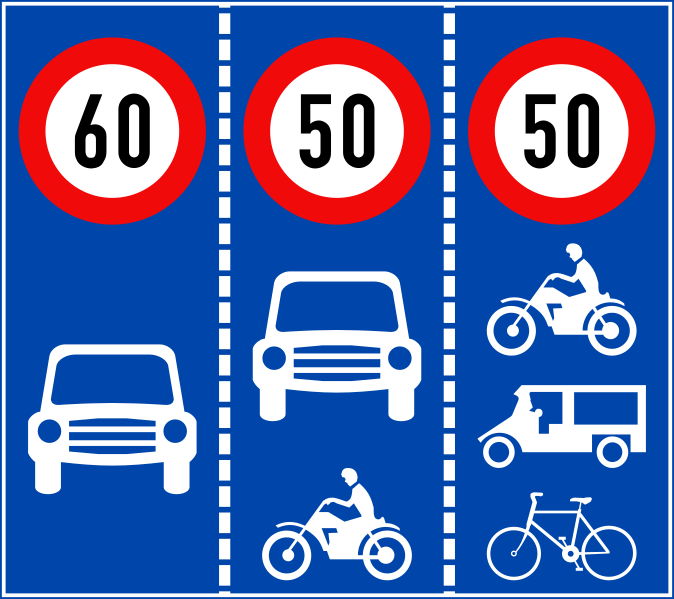
\includegraphics[width=3.5cm]{images/9T5-2-1.png}}	
	\loigiai{
	Với $x$ là tốc độ cho phép của ô tô (xe máy), ta có:
	\begin{listEX}[2]
	\item Ô tô ở làn giữa: $x\leq 50$.
	\item Xe máy ở làn bên phải: $x\leq 50$.
	\end{listEX}
	}
\end{vd}
%%==========Ví dụ 6
\begin{vd}
	Gọi $a$ là số tuối của bạn Na, $b$ là số tuổi của bạn Toàn, biết rằng bạn Toàn lớn tuổi hơn bạn Na. Hãy dùng bất đẳng thức để biểu diễn mối quan hệ về tuổi của hai bạn đó ở hiện tại và sau ba năm nữa.
	\loigiai{
	Bất đẳng thức biểu diễn số tuổi của bạn Toàn và bạn Na là
	$$b>a.$$
	Cộng $3$ vào hai vế của bất đẳng thức $b>a$, ta được bất đẳng thức biểu diễn số tuổi sau ba năm của bạn Toàn và bạn Na
	$$b+3>a+3.$$}
\end{vd}
%%==========Ví dụ 7
\begin{vd}
	Xác định vế trái và vế phải của các bất đẳng thức sau:
	\begin{listEX}[2]
	\item $-2>-7$;
	\item $a^2+1>0$.
	\end{listEX}
	\loigiai{
	\begin{listEX}[2]
	\item Vế trái là $-2$ , vế phải là $-7$.
	\item Vế trái là $a^2+1$, vế phải là $0$.
	\end{listEX}	
	}
\end{vd}
%%==========Ví dụ 8
\begin{vd}
	Trong các cặp bất đẳng thức sau đây, cặp bất đẳng thức nào cùng chiều?
	\begin{listEX}[3]
	\item $3<4$ và $11<23$;
	\item $\sqrt{50}>7$ và $6>\sqrt{34}$.
	\item $\sqrt{17}>\sqrt{13}$ và $\sqrt{82}<\sqrt{97}$.
	\end{listEX}
	\loigiai{
	Cặp bất đẳng thức ở các câu a, b là cặp bất đẳng thức cùng chiều. Cặp bất đẳng thức ở câu c là cặp bất đẳng thức ngược chiều.
	}
\end{vd}
%===============
\begin{dang}{Chứng minh bất đẳng thức}
\end{dang}
%%==========Ví dụ 9
\begin{vd}
	Chứng minh rằng:
	\begin{listEX}[3]
	\item $\dfrac{2\,024}{2\,023}>\dfrac{2021}{2022}$;
	\item $\dfrac{2\,024}{1000}>1{,}9$;
	\item $-\dfrac{2022}{2\,023}>-1{,}1$.
	\end{listEX}
	\loigiai{
	\begin{listEX}
	\item 
	Ta có $\dfrac{2\,024}{2\,023}=1+\dfrac{1}{2\,023}>1$ và $\dfrac{2021}{2022}=1-\dfrac{1}{2022}<1$ nên $\dfrac{2\,024}{2\,023}>\dfrac{2021}{2022}$.
	\item
	Ta có $\dfrac{2\,024}{1000}=2+\dfrac{24}{1000}>2$ và $1{,}9=2-0{,}1<2$ nên $\dfrac{2\,024}{1000}>1{,}9$.
	\item
	Ta có $\dfrac{2022}{2\,024}=1-\dfrac{2}{2\,024}<1$ và $1{,}1=1+0{,}1>1$ nên $\dfrac{2022}{2\,024}<1{,}1$.
	Từ đây suy ra $-\dfrac{2022}{2\,023}>-1{,}1$.
	\end{listEX}
	}
\end{vd}
%%==========Ví dụ 10
\begin{vd}
	Chứng minh rằng
	\begin{listEX}[3]
	\item $\sqrt{11}-\sqrt{3}>\sqrt{10}-\sqrt{3}$;
	\item $2023+\left(-2^{29}\right)>2022+\left(-2^{29}\right)$;	
	\item $\dfrac{2024}{2023}>\dfrac{2025}{2024}$.
	\end{listEX}
	\loigiai{
	\begin{listEX}
	\item Ta có $\sqrt{11}>\sqrt{10}$. Cộng hai vế của bất đẳng thức với $-\sqrt{3}$, ta được: 
	$$\sqrt{11}-\sqrt{3}>\sqrt{10}-\sqrt{3}.$$	
	Vậy $\sqrt{11}-\sqrt{3}>\sqrt{10}-\sqrt{3}.$
	\item
	Ta có $2023>2022$. Cộng hai vế của bất đẳng thức với $-2^{29}$, ta được:
	$$
	2023+\left(-2^{29}\right)>2022+\left(-2^{29}\right) .
	$$
	Vậy $2023+\left(-2^{29}\right)>2022+\left(-2^{29}\right)$.
	\item
	Ta có $\dfrac{1}{2023}>\dfrac{1}{2024}$. Cộng hai vế của bất đẳng thức với $1$, ta được: $$\dfrac{1}{2023}+1>\dfrac{1}{2024}+1 \text{ hay } \dfrac{2024}{2023}>\dfrac{2025}{2024}.$$
	Vậy $\dfrac{2024}{2023}>\dfrac{2025}{2024}$.
	\end{listEX}
	}
\end{vd}
%%==========Ví dụ 11
\begin{vd}
	Cho hai số a và $b$ thoả mãn $a<b$. Chứng tỏ $a+3<b+5$.
	\loigiai{
	Cộng $3$ vào hai vế của bất đẳng thức $a<b$, ta được:
	\begin{align}
	a+3<b+3. 	\tag{1}
	\end{align}
	Cộng $b$ vào hai vế của bất đẳng thức $3<5$, ta được:
	\begin{align}
	3+b<5+b \text { hay } b+3<b+5.	\tag{2}
	\end{align}	
	Từ (1) và (2) suy ra $a+3<b+5$ (tính chất bắc cầu).
	}
\end{vd}
%%==========Ví dụ 12
\begin{vd}
	Cho hai số $m$ và $n$ thoả mãn $m>n$. Chứng tỏ $m+5>n+4$.
	\loigiai{
	Cộng $4$ vào hai vế của bất đẳng thức $m>n$, ta được:
	\begin{align}
	m+4>n+4. 	\tag{1}
	\end{align}
	Cộng $m$ vào hai vế của bất đẳng thức $5>4$, ta được:
	\begin{align}
	m+5>m+4 .	\tag{2}
	\end{align}
	Từ (1) và (2) suy ra $m+5>n+4$ (tính chất bắc cầu).
	}
\end{vd}
%%==========Ví dụ 13
\begin{vd}
	Chứng minh:
	\begin{listEX}[3]
	\item $\left(a+1\right)^2 \leq 2a+2$ với $a^2 \leq 1$.
	\item $\left(a-1\right)^2 \geq 4-2a$ với $a^2 \geq 3$.
	\item $\left(a-1\right)^2 \geq a^2-1$ với $a \leq 1$.
	\end{listEX}
	\loigiai{ 
	\begin{listEX}[1]
	\item 
	Do $a^2 \leq 1$ nên $a^2 +2a+1\leq 1+2a+1$, suy ra $\left(a+1\right)^2 \leq 2a+2$.
	Vậy $\left(a+1\right)^2 \leq 2a+2$.
	\item 
	Do $a^2 \geq 3$ nên $a^2-\left(2a-1\right) \geq 3-\left(2a-1\right) $, suy ra $a^2-2a+1 \geq 4-2a$.
	Vậy $\left(a-1\right)^2 \geq 4-2a$ với $a^2 \geq 3$.
	\item 
	Vì $a \leq 1$ nên $-2a \geq -2$, suy ra $-2a+a^2+1 \geq -2+a^2+1$.
	Do đó $\left(a-1\right)^2 \geq a^2-1$.
	\end{listEX}
	}
\end{vd}
%%==========Ví dụ 14
\begin{vd}
	Cho $a>b$ và $c>d$. Chứng minh $a+c>b+d$.
	\loigiai{
	Do $a>b$ nên $a+c>b+c$.\\
	Lại có $c>d$ nên $b+c>b+d$.\\
	Vậy $a+c>b+d$.
	}
\end{vd}
%%==========Ví dụ 15
\begin{vd}
	Cho $a, b,c, d$ là các số thực dương thỏa mãn $a>b$ và $c>d$. Chứng minh: $ac>bd$. 
	\loigiai{
	Do $a>b$ nên $ac>bc$ (vì $c>0$).\\
	Lại có $c>d$ nên $bc>bd$ (vì $b>0$).\\
	Vậy $ac>bd$.
	}
\end{vd}
%%==========Ví dụ 16
\begin{vd}
	Cho $a<b$. Chứng minh
	\begin{listEX}[3]
	\item $a+b>2a$;
	\item $5a-b<4a$;
	\item $a-1<b+6$.
	\end{listEX}	
	\loigiai{
	\begin{note}
	Để chứng minh $A>B$ ta có thể chứng minh $A-B>0$.
	\end{note}
	Do $a<b$ nên $b-a>0$ và $a-b<0$.
	\begin{listEX}[1]
	\item Xét hiệu $a+b-2a=b-a>0$. Vậy $a+b>2a$.
	\item Xét hiệu $\left(5a-b\right)-4a=a-b<0$. Vậy $5a-b<4a$.
	\item Xét hiệu $\left(b+6\right)-\left(a-1\right)=b-a+7$. \\
	Do $b-a>0$ và $7>0$ nên $\left(b-a\right)+7>0$.\\
	Vậy $\left(b+6\right)-\left(a-1\right)>0$ hay $a-1<b+6$.
	\end{listEX}
	}
\end{vd}
%%==========Ví dụ 17
\begin{vd}
	Cho $a \geq 2b$. Chứng minh:
	\begin{listEX}[2]
	\item $2a-1 \geq a+2b-1$;
	\item $4b+4a \leq 5a+2b$.	
	\end{listEX}
	\loigiai{ 
	\begin{note}
	Để chứng minh $A>B$ ta có thể chứng minh $A-B>0$.
	\end{note}
	Do $a \geq 2b$ nên $a-2b \geq 0$.
	\begin{listEX}[1]	
	\item Xét hiệu $\left(2a-1\right)-\left(a+2b-1\right)=a-2b \geq 0$. Vậy $2a-1 \geq a+2b-1$.
	\item Xét hiệu $\left(5a+2b\right)-\left(4b+4a\right)=a-2b \geq 0$. Vậy $5a+2b \geq 4b+4a$ hay $4b+4a \leq 5a+2b$.
	\end{listEX}
	}
\end{vd}
%%==========Ví dụ 18
\begin{vd}
	Cho $a \geq b$. Chứng minh $5b-2 \leq 5a-2$.
	\loigiai{
	Vì $a \geq b$ nên $5a \geq 5b$.\\
	Do đó $5a-2 \geq 5b-2$ hay $5b-2 \leq 5a-2$.
	Vậy $5b-2 \leq 5a-2$.
	}
\end{vd}
%%==========Ví dụ 19
\begin{vd}Cho $a<b$. Chứng minh
	\begin{listEX}[3]
	\item $\-3a+19>-3b+19$;
	\item $-2a-8>-2b-8$;
	\item $2a+1<2b+1$.
	\end{listEX}
	\loigiai{
	\begin{listEX}[1]
	\item Do $a<b$ nên $-3a>-3b$, suy ra $-3a+19>-3b+19$.
	\item Do $a<b$ nên $-2a>-2b$, suy ra $-2a-8>-2b-8$.
	\item Do $a<b$ nên $2a<2b$, suy ra $2a+1<2b+1$.
	\end{listEX}
	}
\end{vd}
%%==========Ví dụ 20
\begin{vd}
	Cho hai số $a$, $b$ thoả mãn $a^2>b^2>0$. Chứng tỏ $5a^2>4b^2$.
	\loigiai{
	Nhân hai vế của bất đẳng thức $a^2>b^2$ với $5$ , ta được:
	\begin{align}
	5 a^2>5 b^2 .	\tag{3}
	\end{align}
	Vì $b^2>0$ nên khi nhân hai vế của bất đẳng thức $5>4$ với $b^2$, ta được:
	\begin{align}
	5 b^2>4 b^2 .	\tag{4}
	\end{align}
	Từ (3) và (4) suy ra $5 a^2>4 b^2$ (tính chất bắc cầu).
	}
\end{vd}
%%==========Ví dụ 21
\begin{vd}
	Cho hai số $m, n$ thỏa mãn $0<m^2<n^2$. Chứng tỏ $\dfrac{3}{2} m^2<2 n^2$.
	\loigiai{
	Nhân hai vế của bất đẳng thức $m^2<n^2$ với $\dfrac{3}{2}$ , ta được:
	\begin{align}
	\dfrac{3}{2}m^2<\dfrac{3}{2}n^2.	\tag{5}
	\end{align}
	Vì $n^2>0$ nên khi nhân hai vế của bất đẳng thức $\dfrac{3}{2}>2$ với $b^2$, ta được:
	\begin{align}
	\dfrac{3}{2}n^2<2n^2 .	\tag{6}
	\end{align}
	Từ (5) và (6) suy ra $\dfrac{3}{2} m^2<2 n^2$ (tính chất bắc cầu).
	}
\end{vd}
%===============
\begin{dang}{So sánh hai số}
\end{dang}
%%==========Ví dụ 22
\begin{vd}
	Không thực hiện phép tính, hãy so sánh:
	\begin{listEX}[2]
	\item $2\,023+(-19)$ và $2\,024+(-19)$;	
	\item $19+2\,023$ và $-31+2\,023$;
	\item $\sqrt{2}+2$ và $4$;
	\item $-3+23^{50}$ và $-2+23^{50}$
	\end{listEX}	
	\loigiai{
	\begin{listEX}
	\item
	Vì $2\,023<2\,024$ nên
	$$2\,023+(-19)<2\,024+(-19)\,\,\ \leftarrow\text{cộng vào hai vế với cùng một số }-19.$$
	Vậy $2\,023+(-19)<2\,024+(-19)$.
	\item 
	Vì $19>-31$ nên
	$$19+2\,023>-31+2\,023\,\,\ \leftarrow\text{cộng vào hai vế với cùng một số } 2\,023.$$
	Vậy $19+2\,023>-31+2\,023$.
	\item 
	Vì $\sqrt{2}<2$ nên
	$$\sqrt{2}+2<2+2\,\,\ \leftarrow\text{cộng vào hai vế với cùng một số } 2.$$
	Vậy $\sqrt{2}+2<4$.
	\item
	Ta có $-3<-2$ nên
	$$-3+23^{50}<-2+23^{50}\,\,\ \leftarrow\text{Cộng hai vế của bất đẳng thức với } 23^{50}.$$
	Vậy $-3+23^{50}<-2+23^{50}$.
	\end{listEX}
	}
\end{vd}
%%==========Ví dụ 23
\begin{vd}%[8D4B2]
	Cho $a<b$, hãy so sánh:
	\begin{enumEX}{2}
	\item $a-3$ và $b-3$;
	\item $-5a+1$ và $-5b+1$.
	\end{enumEX}
	\loigiai{
	\begin{enumerate}
	\item Ta có $a<b$. Cộng thêm $-3$ vào hai vế ta được $a-3<b-3$.
	\item Ta có $a<b$. Nhân hai vế với $-5$ ta được $-5a>-5b$. Cộng thêm $1$ vào hai vế, ta được $-5a+1>-5a+1$.
	\end{enumerate}
	}
\end{vd}
%%==========Ví dụ 24
\begin{vd}%[8D4B1]
	Cho số $a$ bất kì, hãy so sánh:
	\begin{enumEX}{2}
	\item $a$ và $a-4$;
	\item $a-7$ và $a+5$.
	\end{enumEX}
	\loigiai{
	\begin{enumerate}
	\item Ta có $0>-4$. Cộng thêm $a$ vào hai vế ta được $a>a-4$.
	\item Ta có $-7<5$. Cộng thêm $a$ vào hai vế ta được $a-7<a+5$.
	\end{enumerate}
	}
\end{vd}
%%==========Ví dụ 25
\begin{vd}
	Thay \boxEX[15pt]{?} trong các biểu thức sau bởi dấu thích hợp ($<$, $>$) để được khẳng định đúng.
	\begin{listEX}[2]
	\item $3\cdot(-7)\boxEX[15pt]{?} 3\cdot(-5)$;
	\item $(-3)\cdot(-7) \boxEX[15pt]{?}(-3)\cdot(-5)$.
	\end{listEX}
	\loigiai{
	\begin{listEX}
	\item Vì $-7<-5$ và $3>0$ nên $3 \cdot(-7)\boxEX[15pt]{$<$}3 \cdot(-5)$. $\leftarrow$ nhân cả hai vế của bất đẳng thức với số dương.
	\item Vì $-7<-5$ và $-3<0$ nên $(-3) \cdot(-7)\boxEX[15pt]{$>$}(-3) \cdot(-5)$. $\leftarrow$ nhân cả hai vế của bất đẳng thức với số âm.
	\end{listEX}
	}
\end{vd}
%%==========Ví dụ 26
\begin{vd}
	Thay \boxEX[15pt]{?} trong các biểu thức sau bởi dấu thích hợp ($<$, $>$) để được khẳng định đúng.
	\begin{listEX}[2]
	\item $13\cdot(-10{,}5) \boxEX[15pt]{?} 13\cdot 11{,}2$;
	\item $(-13)\cdot(-10{,}5) \boxEX[15pt]{?}(-13)\cdot 11{,}2$.
	\end{listEX}	
	\loigiai{
	\begin{listEX}
	\item Vì $-10{,}5<11{,}2$ và $13>0$ nên $13 \cdot(-10{,}5)\boxEX[15pt]{$<$}13 \cdot 11{,}2$. $\leftarrow$ nhân cả hai vế của bất đẳng thức với số dương.
	\item Vì $-10{,}5<11{,}2$ và $-13<0$ nên $(-13) \cdot(-10{,}5)\boxEX[15pt]{$>$}(-13) \cdot 11{,}2$. $\leftarrow$ nhân cả hai vế của bất đẳng thức với số âm.
	\end{listEX}
	}
\end{vd}
%%==========Ví dụ 27
\begin{vd}
	Không thực hiện phép tính, hãy so sánh: 
	\begin{listEX}[2]
	\item $1962\cdot 12$ và $1963\cdot 12$.
	\item $47\cdot (-19)$ và $50\cdot (-19)$.
	\item $(-163)\cdot (-75)^{15}$ và $(-162) \cdot(-75)^{15}$.
	\item $m$ và $n$, biết $-10 m \leq-10 n$.
	\end{listEX}
	\loigiai{
	\begin{listEX}
	\item
	Ta có $1962<1963$. Nhân hai vế của bất đẳng thức với $12$ , ta được:
	$$	1962\cdot 12<1963\cdot 12 .	$$
	\item
	Ta có $47<50$. Nhân hai vế của bất đẳng thức với $-19$ , ta được:
	$$	47\cdot (-19)>50 \cdot (-19) .	$$
	\item
	Ta có $-163< -162$. Nhân hai vế của bất đẳng thức với $(-75)^{15}$ , ta được:
	$$	(-163)\cdot (-75)^{15} > (-162) \cdot(-75)^{15}	.	$$
	\item
	Nhân hai vế của bất đẳng thức $-10 m \leq-10 n$ với $\left (-\dfrac{1}{10}\right )$, ta được
	\allowdisplaybreaks{\begin{eqnarray*}
	\left (-\dfrac{1}{10}\right )\cdot (-10 m) &\geq& \left (-\dfrac{1}{10}\right )\cdot(-10 n) \\
	m&\ge& n.
	\end{eqnarray*} }
	\end{listEX}
	}
\end{vd}
%%==========Ví dụ 28
\begin{vd}%[8D4K2]
	Cho số $m$ bất kì, hãy so sánh $m^2$ và $m$.
	\loigiai{
	\begin{itemize}
	\item Trường hợp $m<0$ thì $m^2>0$, do đó $m^2>m$.
	\item Trường hợp $m=0$ thì $m^2=0$, do đó $m^2=m$.
	\item Trường hợp $0<m<1$. Nhân hai vế cho $m>0$ ta được $m^2<m$.
	\item Trường hợp $m=1$ thì $m^2=1$, do đó $m^2=m$.
	\item Trường hợp $m>1$. Nhân hai vế với $m$ ta được $m^2>m$.
	\end{itemize}
	Tóm lại:
	\begin{itemize}
	\item [-] Nếu $m=0$ hoặc $m=1$ thì $m^2=m$.
	\item [-] Nếu $m<0$ hoặc $m>1$ thì $m^2>m$.
	\item [-] Nếu $0<m<1$ thì $m^2<m$.
	\end{itemize}
	}
\end{vd}
%==================
%===================
\begin{dang}{Bài toán thực tế}
\end{dang}
%%==========Ví dụ 29
\begin{vd}
	Một nhà tài trợ dự kiến tổ chức một buổi đi dã ngoại tập thể nhằm giúp các bạn học sinh vùng cao trải nghiệm thực tế tại một trang trại trong $1$ ngày (từ $14$h$00$ ngày hôm trước đến $12$h$00$ ngày hôm sau). Cho biết số tiền tài trợ dự kiến là $30$ triệu đồng và giá thuê các dịch vụ và phòng nghỉ là $17$ triệu đồng $1$ ngày, giá mỗi suất ăn trưa, ăn tối là $60\,000$ đồng và mỗi suất ăn sáng là $30\,000$ đồng. Hỏi có thể tổ chức cho nhiều nhất bao nhiêu bạn tham gia được?
	\loigiai{
	Gọi số bạn tham gia là $x$ ($x\in \mathbb{N^*}$).\\
	Theo đề bài ta có $17\,000\,000+ (60\,000+30\,000)x\leq 30\,000\,000$ hay $90\,000x\leq 13\,000\,000$.\\
	Suy ra $x\leq \dfrac{1300}{9}=144{,}(4)$.\\
	Vậy có thể tổ chức nhiều nhất cho $144$ bạn tham gia.
	}
\end{vd}
%%==========Ví dụ 30
\begin{vd}
	Một ca nô đi xuôi dòng trong $2$ giờ $30$ phút. Biết rằng tốc độ của ca nô khi nước yên lặng không quá $40$ km/h và tốc độ của dòng nước là $6$ km/h. Chứng minh quãng đường ca nô đi được trong thời gian trên không vượt quá $115$ km/h.
	\loigiai{
	Gọi tốc độ của ca nô khi nước yên lặng là $x$ (km/h) ($x>6$). Tốc độ ca nô đi xuôi dòng là $x+6$ (km/h).\\
	Ta có $x \leq 40$ nên $x+6 \leq 40+6$, tức là $x+6 \leq 46$.\\
	Gọi $s$ (km) là quãng đường ca nô đi được trong $2$ giờ $30$ phút = $2{,}5$ giờ.\\
	Ta có $s=2{,}5 \cdot (x+6)$ (km). Do $x+6\leq 46$ nên $2{,}5 \cdot (x+6) \leq 2{,}5 \cdot 46 = 115$ hay $s \leq 115$.\\
	Vậy quãng đường ca nô đi đi được trong $2$ giờ $30$ phút không vượt quá $115$ km.
	}
\end{vd}
%%==========Ví dụ 31
\begin{vd}
	Chỉ số cơ thể, thường được biết đến với tên viết tắt \textbf{BMI} (tiếng anh là \textit{Body Mass Index}) cho phép đánh giá thể trạng của một người là gầy, bình thường hay béo. Chỉ số cơ thể của người được tính theo công thức sau $BMI=\dfrac{m}{h^2}$, trong đó $m$ là khối lượng lượng cơ thể tính theo kilôgam, $h$ là chiều cao tính theo mét. Căn cứ vào bảng đánh giá thể trạng ở người lớn theo BMI đối với khu vực châu Á - Thái Bình Dương, một người đàn ông có $BMI\geq 30$ sẽ bị béo phì độ II (trung bình) hoặc độ III (nặng), người đó cần phải có biện pháp tập thể dục, thể thao, thay đổi chế độ dinh dưỡng để có được cơ thể khỏe mạnh (\textit{Nguồn: Toán 7---Tập Hai, NXB Giáo dục Việt Nam, năm $2017$}). Bác Dũng có chiều cao $1{,}65$ và cân nặng ít nhất là $82$ kg. Hỏi bác Dũng có bị béo phì độ II hoặc độ III không? 
	\loigiai{
	Gọi $m$ (kg) là khối lượng cơ thể của bác Dũng, $h$ (m) là chiều cao của bác Dũng.\\
	Theo giả thiết, ta có $m\geq 82$; $h=1{,}65$. Do đó chỉ số BMI của bác Dũng là\\
	$$ BMI=\dfrac{m}{(1{,}65)^2}=\dfrac{m}{2{,}7225}$$
	Do $m\geq82$ nên $\dfrac{m}{2{,}7225}\geq \dfrac{82}{2{,}7225}$.\\
	Vì $\dfrac{82}{2{,}7225} \approx 30{,}11938$ và $30{,}11938>30$ nên $\dfrac{m}{2{,}7225}>30$.\\
	Như vậy bác Dũng có thể đã bị béo phì độ II hoặc độ III.
	}
\end{vd}
%==================
\begin{dang}{Áp dụng bất đẳng thức để tìm giá trị lớn nhất, giá trị nhỏ nhất của một biểu thức}
	\begin{itemize}
	\item Nếu $f(x)\geq k$ ($k$ là hằng số) và dấu ``='' xảy ra khi và chỉ khi $x=a$ thì giá trị nhỏ nhất của $f(x)$ là $k$ khi và chỉ khi $x=a$.\\
	Ta viết $\min f(x)=k$ khi và chỉ khi $x=a$.
	\item Nếu $f(x)\leq k$ ($k$ là hằng số) và dấu ``='' xảy ra khi và chỉ khi $x=a$ thì giá trị lớn nhất của $f(x)$ là $k$ khi và chỉ khi $x=a$.\\
	Ta viết $\max f(x)=k$ khi và chỉ khi $x=a$.
	\end{itemize}
\end{dang}
%%==========Ví dụ 32
\begin{vd}%[8D4K2]
	Tìm giá trị nhỏ nhất của biểu thức $A=x^2-6x+10$.
	\loigiai{
	Ta có $A=x^2-6x+10=x^2-6x+9+1=(x-3)^2+1\geq 1$ (dấu ``='' xảy ra khi và chỉ khi $x=3$).\\
	Do đó $\min A=1$ khi và chỉ khi $x=3$.	
	}
\end{vd}
%%==========Ví dụ 33
\begin{vd}%[8D4K2]
	Tìm giá trị nhỏ nhất của biểu thức $B=5x^2-10x+3$.
	\loigiai{
	Ta có 
	$B=5x^2-10x+3=5x^2-10x+5-2=5(x-1)^2-2\geq -2$ (dấu ``='' xảy ra khi và chỉ khi $x=1$).\\
	Vậy $\min B=-2$ khi và chỉ khi $x=1$.
	}
\end{vd}
%%==========Ví dụ 34
\begin{vd}%[8D4G2]
	Tìm giá trị lớn nhất của biểu thức $C=-x^2+5x-4$.
	\loigiai{
	Ta có
	\begin{eqnarray*}
	C&=& -x^2+5x-4=-(x^2-5x+4)=-\left(x^2-2\cdot \dfrac{5}{2}x+\dfrac{25}{4}-\dfrac{25}{4}+4\right)\\
	&=& -\left[ \left(x-\dfrac{5}{2} \right)^2-\dfrac{9}{4} \right]=-\left( x-\dfrac{5}{2} \right)^2+\dfrac{9}{4}\leq \dfrac{9}{4}\; \text{ (dấu ``='' xảy ra khi và chỉ khi } x=\dfrac{5}{2}).
	\end{eqnarray*}
	Vậy $\max C=\dfrac{9}{4}$ khi $x=\dfrac{5}{2}$.
	}
\end{vd}
%%==========Ví dụ 35
\begin{vd}%[8D4K2]
	Tìm giá trị nhỏ nhất của biểu thức $E=2x^2+8x+y^2-10y+43$.
	\loigiai{
	Ta có
	\begin{eqnarray*}
	E&=& 2x^2+8x+y^2-10y+43=2x^2+8x+8+y^2-10y+25+10\\
	&=& 2(x^2+4x+4)+(y-5)^2+10=2(x+2)^2+(y-5)^2+10\geq 10.
	\end{eqnarray*}	
	(dấu ``='' xảy ra khi và chỉ khi $x=-2$ và $y=5$).\\
	Vậy $\min E=10$ khi và chỉ khi $x=-2$ và $y=5$.
	}
\end{vd}
%%==========Ví dụ 36
\begin{vd}%[8D4K2]
	Tìm giá trị nhỏ nhất của biểu thức $F=\dfrac{2x-1}{x^2+2}$.
	\loigiai{
	Ta có $$F=	\dfrac{2x-1}{x^2+2}=\dfrac{x^2+2x+1-x^2-2}{x^2+2}=\dfrac{(x+1)^2}{x^2+2}-\dfrac{x^2+2}{x^2+2}=\dfrac{(x+1)^2}{x^2+2}-1\geq -1.$$
	(dấu ``='' xảy ra khi và chỉ khi $x=-1$).\\
	Vậy $\min F=-1$ khi và chỉ khi $x=-1$. 
	}
\end{vd}
%%%%%%%%%%%%%%%%%%%%
\subsection{Bài tập vận dụng}
%%==========Bài 1
\begin{bt}
Dùng kí hiệu để viết bất đẳng thức tương ứng với mỗi trường hợp sau:
\begin{listEX}[2]
\item $x$ nhỏ hơn hoặc bằng $-2$;
\item $m$ là số âm;
\item $y$ là số dương;
\item $p$ lớn hơn hoặc bằng $2\,024$.
\end{listEX}
\loigiai{
\begin{listEX}[4]
	\item $x\leq -2$.
	\item $m<0$.
	\item $y>0$.
	\item $p\geq 2\,024$.
\end{listEX}
}
\end{bt}
%%==========Bài 2
\begin{bt}
Viết một bất đẳng thức phù hợp trong mỗi trường hợp sau:
\begin{listEX}
\item Bạn phải ít nhất $18$ tuổi mới được phép lái ô tô;
\item Xe buýt chở được tối đa $45$ người;
\item Mức lương tối thiểu cho một giờ làm việc của người lao động là 
$20\,000$ đồng.
\end{listEX}
\loigiai{
\begin{listEX}
	\item Với $t$ là số tuổi, ta có bất đẳng thức: $t\geq 18$.
	\item Với $x$ là số người xe buýt chở được, ta có bất đẳng thức: $x\leq 45$.
	\item Với $y$ là mức lương tối thiểu cho một giờ làm việc của người lao động, ta có bất đẳng thức: $y\geq 20\,000$.
\end{listEX}
}
\end{bt}
%%==========Bài 3
\begin{bt}
	Dùng các kí hiệu $>$, $<$, $\geq$, $\leq$ để diễn tả:
	\begin{enumerate}
	\item Tốc độ $v$ đúng quy định với biển báo giao thông ở hình dưới.
	\item Trọng tải $P$ của toàn bộ xe khi đi qua cầu đúng quy định với biển báo giao thông ở Hình $4b$.
	\end{enumerate}
	\begin{center}
	\begin{tikzpicture}[scale=0.8,>=stealth, font=\footnotesize,line join=round,line cap=round,transform shape]
	%\draw[thick] (0,0) circle (1.85 cm);
	\fill[red] (0,0) circle (1.8 cm);
	\fill[white] (0,0) circle (1.4 cm);
	\node at (0,0){\bfseries\fontfamily{anttlc}\fontsize{55}{40}\selectfont{70}};
	\node at ($(0,0)+(0,-2.2)$){Hình a)};
	\end{tikzpicture}
	\hspace*{2cm}
	\begin{tikzpicture}[scale=0.8,>=stealth, font=\footnotesize,line join=round,line cap=round,transform shape]
	%\draw[thick] (0,0) circle (1.85 cm);
	\fill[red] (0,0) circle (1.8 cm);
	\fill[white] (0,0) circle (1.4 cm);
	\node at (-0.2,0){\bfseries\fontfamily{anttlc}\fontsize{50}{40}\selectfont{10}};
	\node at (0.8,0.5){\bfseries\rmfamily\fontsize{30}{40}\selectfont{t}};
	\node at ($(0,0)+(0,-2.2)$){Hình b)};
	\end{tikzpicture}
	\end{center}
	\loigiai{
	\begin{listEX}[2]
	\item $v\leq 70$.
	\item $P\leq 10$.
	\end{listEX}
	}	
\end{bt}
%%==========Bài 4
\begin{bt}
	Hãy chỉ ra các bất đẳng thức diễn tả mỗi khẳng định sau:
	\begin{listEX}[2]
	\item $m$ lớn hơn $8$;
	\item $n$ nhỏ hơn $21$;
	\item $x$ nhỏ hơn hoặc bằng $4$;
	\item $y$ lớn hơn hoặc bằng $0$.
	\end{listEX}
	\loigiai{
	\begin{listEX}[4]
	\item $m>8$.
	\item $n<21$.
	\item $x\leq 4$.	
	\item $y \geq 0$.
	\end{listEX}
	}	
\end{bt}
%%==========Bài 5
\begin{bt}
	Hãy cho biết các bất đẳng thức được tạo thành khi:
	\begin{enumerate}
	\item Cộng hai vế của bất đẳng thức $m>5$ với $-4$;
	\item Cộng hai vế của bất đẳng thức $x^2 \leq y+1$ với $9$;
	\item Nhân hai vế của bất đẳng thức $x>1$ với $3$, rồi tiếp tục cộng với $2$;
	\item Cộng vào hai vế của bất đẳng thức $m \leq -1$ với $-1$, rồi tiếp tục cộng với $-7$.
	\end{enumerate}
	\loigiai{
	\begin{enumerate}
	\item Cộng hai vế của bất đẳng thức $m>5$ với $-4$ ta được
	\allowdisplaybreaks{\begin{eqnarray*}
	m+(-4)&>& 5+(-4)\\
	m-4&>& 1.
	\end{eqnarray*} }
	\item Cộng hai vế của bất đẳng thức $x^2 \leq y+1$ với $9$ ta được
	\allowdisplaybreaks{\begin{eqnarray*}
	x^2+9 &\leq& y+1+9\\
	x^2+9 &\leq& y+10.
	\end{eqnarray*} }
	\item Nhân hai vế của bất đẳng thức $x>1$ với $3$ ta được
	\allowdisplaybreaks{\begin{eqnarray*}
	x\cdot 3 &>&1\cdot 3\\
	3x &>&3.
	\end{eqnarray*} }
	Cộng hai vế của bất đẳng thức $3x >3$ với $2$ ta được
	\allowdisplaybreaks{\begin{eqnarray*}
	3x +2&>&3+2\\
	3x +2&>&5.
	\end{eqnarray*} }
	\item Cộng vào hai vế của bất đẳng thức $m \leq -1$ với $-1$ ta được
	\allowdisplaybreaks{\begin{eqnarray*}
	m+(-1) &\leq& -1+(-1)\\
	m-1 &\leq& -2.
	\end{eqnarray*} }
	Cộng hai vế của bất đẳng thức $m-1\leq -2$ với $-7$ ta được
	\allowdisplaybreaks{\begin{eqnarray*}
	m-1 +(-7)&\leq -2+(-7)\\
	m-8&\leq -9.
	\end{eqnarray*} }
	\end{enumerate}
	}	
\end{bt}
%%==========Bài 6
\begin{bt}
Cho $a<b$, hãy so sánh:
\begin{listEX}[2]
	\item $5a+7$ và $5b+7$;
	\item $-3a-9$ và $-3b-9$.
\end{listEX}
\loigiai{
\begin{listEX}
	\item 
	Vì $a<b$ và $5>0$ nên $5a<5b$.\\
	Cộng hai vế của bất đẳng thức trên với $7$ ta được
	$5a+7<5b+7.$
	\item 
	Vì $a<b$ và $-3<0$ nên $-3a>-3b$.\\
	Cộng hai vế của bất đẳng thức trên với $-9$ ta được
	$-3a-9>-3b-9.$
\end{listEX}
}
\end{bt}
%%==========Bài 7
\begin{bt}
So sánh hai số $a$ và $b$, nếu:
\begin{listEX}[2]
	\item $a+1\,954<b+1\,954$;
	\item $-2a>-2b$.
\end{listEX}
\loigiai{
\begin{listEX}
	\item Ta có $a+1\,954<b+1\,954$.\hfill (1)\\
	Cộng cả hai vế của bất đẳng thức (1) với $-1\,954$ ta được
	$$a+1\,954-1\,954<b+1\,954-1954.$$
	Hay $a<b$.
	\item 
	Ta có $-2a>-2b$.\hfill (2)\\
	Nhân cả hai vế của bất đẳng thức (2) với $-\dfrac{1}{2}$ ta được
	$$-2a\cdot\dfrac{-1}{2}<-2b\cdot\dfrac{-1}{2}$$
	Hay $a<b$.
\end{listEX}
}
\end{bt}
%%==========Bài 8
\begin{bt}
	So sánh hai số $x$ và $y$ trong mỗi trường hợp sau:
	\begin{listEX}[4]
	\item $x+5>y+5$;
	\item $-11x \leq-11 y$;
	\item $3x-5<3y-5$;
	\item $-7x+1>-7y+1$.	
	\end{listEX}
	\loigiai{
	\begin{enumerate}
	\item Cộng hai vế của bất đẳng thức $x+5>y+5$ với $-5$ ta được
	\allowdisplaybreaks{\begin{eqnarray*}
	x+5+(-5) &>& y+5+(-5)\\
	x&>& y.
	\end{eqnarray*} }
	Vậy $x>y$.
	\item Nhân hai vế của bất đẳng thức $-11x \leq-11 y$ với $\dfrac{-1}{11}$ ta được
	\allowdisplaybreaks{\begin{eqnarray*}
	-11x \cdot \left(\dfrac{-1}{11}\right) &\geq& -11 y \cdot \left(\dfrac{-1}{11}\right) \\
	x &\geq& y.
	\end{eqnarray*} }
	Vậy $x \geq y$.
	\item Cộng hai vế của bất đẳng thức $3x-5<3y-5$ với $5$ ta được
	\allowdisplaybreaks{\begin{eqnarray*}
	3x-5+5 &<& 3y-5+5 \\
	3x&<&3y. 
	\end{eqnarray*} }
	Tiếp tục nhân hai vế của bất đẳng thức $3x<3y$ với $\dfrac{1}{3}$ ta được
	\allowdisplaybreaks{\begin{eqnarray*}
	3x\cdot \left(\dfrac{1}{3}\right)&<& 3y\cdot \left(\dfrac{1}{3}\right) \\
	x &<& y.
	\end{eqnarray*} }
	Vậy $x<y$.
	\item Cộng hai vế của bất đẳng thức $-7x+1>-7y+1$ với $-1$ ta được
	\allowdisplaybreaks{\begin{eqnarray*}
	-7x+1+(-1)&>&-7y+1+(-1) \\
	-7x&>&-7y.
	\end{eqnarray*} }
	Tiếp tục nhân hai vế của bất đẳng thức $-7x>-7y$ với $\dfrac{-1}{7}$ ta được
	\allowdisplaybreaks{\begin{eqnarray*}
	-7x\cdot \left(\dfrac{-1}{7}\right) &<& -7y\cdot \left(\dfrac{-1}{7}\right) \\
	x &<& y.
	\end{eqnarray*} }
	Vậy $x<y$.
	\end{enumerate}
	}	
\end{bt}
%%==========Bài 9
\begin{bt}%[8D4K1]
	So sánh $2m$ và $m$.
	\loigiai{
	Bạn phải xét ba trường hợp: $m=0$; $m>0$; $m<0$.
	\begin{itemize}
	\item Nếu $m=0$ thì $2m=m=0$.
	\item Nếu $m>0$ thì $2m>m$.
	\item Nếu $m<0$ thì $2m<m$.
	\end{itemize}	
	}
\end{bt}
%%==========Bài 10
\begin{bt}
	Không thực hiện phép tính, hãy chứng minh:
	\begin{listEX}[2]
	\item $2\cdot(-7)+2\,023<2 \cdot(-1)+2\,023$;
	\item $(-3)\cdot(-8)+1\,975>(-3) \cdot(-7)+1\,975$.
	\end{listEX}
	\loigiai{
	\begin{listEX}
	\item
	Vì $-7<-1$ và $2>0$ nên $2\cdot(-7)<2\cdot (-1)$.\\
	Cộng hai vế của bất đẳng thức trên với $2\,023$ ta được
	$2\cdot(-7)+2\,023<2 \cdot(-1)+2\,023.$
	\item
	Vì $-8<-7$ và $-3<0$ nên $(-3)\cdot(-8)>(-3)\cdot (-7)$.\\
	Cộng hai vế của bất đẳng thức trên với $2\,023$ ta được
	$(-3)\cdot(-8)+2\,023>2 \cdot(-7)+2\,023.$
	\end{listEX}
	}
\end{bt}
%%==========Bài 11
\begin{bt}
Chứng minh rằng:
\begin{listEX}[2]
\item $-\dfrac{2\,023}{2\,024}>-\dfrac{2\,024}{2\,023}$;
\item $\dfrac{34}{11}>\dfrac{26}{9}$.
\end{listEX}
\loigiai{
\begin{listEX}
	\item 
	Ta có $\dfrac{2\,023}{2\,024}=1-\dfrac{1}{2\,024}<1$ và $\dfrac{2\,024}{2\,023}=1+\dfrac{1}{2\,023}>1$ nên $\dfrac{2\,023}{2\,024}<\dfrac{2\,024}{2\,023}$.\\
	Suy ra $-\dfrac{2\,023}{2\,024}>-\dfrac{2\,024}{2\,023}$.
	\item 
	Ta có $\dfrac{34}{11}=3+\dfrac{1}{11}>3$ và $\dfrac{26}{9}=3-\dfrac{1}{9}<3$ nên $\dfrac{34}{11}>\dfrac{26}{9}$.\\
	Vậy $\dfrac{34}{11}>\dfrac{26}{9}$.
\end{listEX}
}
\end{bt}
%%==========Bài 12
\begin{bt}
	Chứng minh
	\begin{listEX}[2]
	\item $\sqrt{29}-\sqrt{6}>\sqrt{28}-\sqrt{6}$;
	\item $26{,}2<2a+3{,}2<26{,}4$ với $11{,}5<a<11{,}6$.
	\end{listEX}
	\loigiai{
	\begin{listEX}[2]
	\item
	Ta có\\
	$\sqrt{29}>\sqrt{28}$ (vì $29>28$)\\
	Cộng hai vế cho $-\sqrt{6}$ ta được\\
	$\sqrt{29}-\sqrt{6}>\sqrt{28}-\sqrt{6}$.\\
	Vậy $\sqrt{29}-\sqrt{6}>\sqrt{28}-\sqrt{6}$.
	\item
	Ta có $11{,}5<a<11{,}6$\\
	Nhân $2$ vào hai vế ta được\\
	$23<2a<23,2$\\
	Cộng $3{,2}$ vào hai vế ta được\\
	$26{,}2<2a+3{,}2<26{,}4$.
	\end{listEX}	
	}
\end{bt}
%%==========Bài 13
\begin{bt}
	Chứng minh
	\begin{listEX}[2]
	\item $\dfrac{1}{1\cdot2}+\dfrac{1}{2\cdot3}+\dfrac{1}{3\cdot4}<a^2+\dfrac{4}{5}$ với $a\neq 0$;
	\item $2m+4>2n+3$ với $m>n$.
	\end{listEX}
	\loigiai{
	\begin{listEX}
	\item
	Ta có $\dfrac{1}{1\cdot2}+\dfrac{1}{2\cdot3}+\dfrac{1}{3\cdot4} = 1-\dfrac{1}{2}+\dfrac{1}{2}-\dfrac{1}{3}+\dfrac{1}{3}-\dfrac{1}{4}=1-\dfrac{1}{4}=\dfrac{1}{4}=\dfrac{5}{20}$.\\
	Mà $\dfrac{4}{5}=\dfrac{16}{20}$ nên $\dfrac{5}{20}<\dfrac{16}{20}$.\\
	Do đó $\dfrac{1}{4}<\dfrac{4}{5}< a^2+\dfrac{4}{5}$ với $a\neq 0$.\\
	Vậy $\dfrac{1}{1\cdot2}+\dfrac{1}{2\cdot3}+\dfrac{1}{3\cdot4}<a^2+\dfrac{4}{5}$ với $a\neq 0$.
	\item $2m+4>2n+3$ với $m>n$.\\
	Ta có $m>n$\\
	Nhân $2$ vào hai vế\\ Ta được
	$2m>2n$\\
	Cộng $4$ vào hai vế\\ Ta được
	$2m+4>2n+3$.
	\end{listEX}
	}
\end{bt}
%%==========Bài 14
\begin{bt}
	\textbf{}
	\begin{listEX}[2]
	\item Cho $a>b>0$. Chứng minh $\dfrac{1}{a}<\dfrac{1}{b}$.
	\item Áp dụng kết quả trên, hãy so sánh $\dfrac{2022}{2023}$ và $\dfrac{2023}{2024}$.
	\end{listEX}
	\loigiai{
	\begin{listEX}
	\item Cho $a>b>0$. Chứng minh $\dfrac{1}{a}<\dfrac{1}{b}$.
	Ta có $a>b>0$ nên $ab>0$ do đó $\dfrac{1}{ab}>0$.\\
	Nhân cả hai vế của bất đẳng thức $a>b$ cho $\dfrac{1}{ab}$\\
	Ta được $a\cdot\dfrac{1}{ab}>b\cdot\dfrac{1}{ab}$ hay $\dfrac{1}{b}>\dfrac{1}{a}$.\\
	Do đó $\dfrac{1}{a}<\dfrac{1}{b}$.
	\item Áp dụng kết quả trên, hãy so sánh $\dfrac{20022}{2023}$ và $\dfrac{2023}{2024}$.\\
	Ta có \\
	$\dfrac{2022}{2023}=1-\dfrac{1}{2023}$.\\ $\dfrac{2023}{2024}=1-\dfrac{1}{2024}$.\\
	Vì $\dfrac{1}{2023}>\dfrac{1}{2024}$ nên $1-\dfrac{1}{2023}<1-\dfrac{1}{2024}$ hay $\dfrac{2022}{2023}<\dfrac{2023}{2024}$.
	\end{listEX}
	}
\end{bt}
%%==========Bài 15
\begin{bt}
	Chứng minh $x^2+y^2\geq 2xy$ với mọi số thực $x, y$.
	\loigiai{
	Ta có $(x-y)^2 \geq 0$ với mọi số thực $x, y$\\
	Suy ra $x^2+y^2\geq 2xy$\\
	Suy ra $x^2+y^2-2xy\geq 0$.\\
	Dấu \lq \lq$=$\rq\rq \,khi $(x-y)^2=0$ suy ra $x=y$.
	}
\end{bt}
%%==========Bài 16
\begin{bt}%[8D4B2]
	Cho $a+3>b+3$. Chứng minh rằng $-2a+1<-2b+1$.
	\loigiai{
	Ta có $a+3>b+3 \Rightarrow a>b \Rightarrow -2a<-2b \Rightarrow -2a+1<-2b+1$.
	}
\end{bt}
%%==========Bài 17
\begin{bt}%[8D4B2]
	Cho $a$, $b$, $c$ là ba cạnh của một tam giác. Chứng minh rằng $a<\dfrac{a+b+c}{2}$.
	\loigiai{
	Ta có $a<b+c$ (bất đẳng thức tam giác).
	$$\Rightarrow 2a<a+b+c \Rightarrow a<\dfrac{a+b+c}{2}.$$
	}
\end{bt}
%%==========Bài 18
\begin{bt}%[8D4K2]
	Tìm giá trị nhỏ nhất của các biểu thức: $A=2x^2+28x+101$.
	\loigiai{
	Ta có $A=2x^2+28x+98+3=2(x+7)^2+3\geq 3$. Do đó $\min A=3$ khi và chỉ khi $x=-7$.
	}
\end{bt}
%%==========Bài 19
\begin{bt}%[8D4G2]
	Tìm giá trị lớn nhất của các biểu thức: $C=-x^2+5x$.
	\loigiai{
	Ta có
	\begin{eqnarray*}
	C&=&-x^2+5x=-(x^2-5x)\\
	&=&-\left( x^2-2\cdot \dfrac{5}{2}x+\dfrac{25}{4}-\dfrac{25}{4} \right)\\
	&=&-\left[ \left( x-\dfrac{5}{2} \right)^2-\dfrac{25}{4} \right]\\
	&=&-\left( x-\dfrac{5}{2} \right)^2+\dfrac{25}{4}\leq \dfrac{25}{4}.
	\end{eqnarray*}
	Vậy $\max C=\dfrac{24}{5}$ khi và chỉ khi $x=\dfrac{5}{2}$.
	}
\end{bt}